\documentclass[border=4pt,12pt]{standalone}
% House style for redrawn exam diagrams (diagram-v4: 0.4pt lines, filled -latex arrows, fine dashes; stipple and hatching drawn as real dots/lines (no PDF/SVG patterns, so they render in every browser and at any scale); transparent background). Every figure \input's this.
\usepackage{amsmath,amssymb}
\usepackage{txfonts}
\usepackage{pdfrender,xcolor}
% \halo{text}: label on shading. The shading stops just around each letter's outline (a thin knock-out that follows the
% glyphs, like the papers' typesetting), never a box. Owner: "I don't want a box around the text".
\newcommand{\halo}[1]{\leavevmode\rlap{\pdfrender{TextRenderingMode=2,LineWidth=2.2pt,LineJoinStyle=1,StrokeColor=white,FillColor=white}#1}#1}
\usepackage{tikz,pgfplots}
\pgfplotsset{compat=1.18}
\usetikzlibrary{arrows.meta,calc,angles,quotes,patterns,patterns.meta,intersections,positioning,decorations.markings,shapes.geometric}
% Stipple and hatching are drawn as actual dots / lines clipped to the region (path picture), NOT as pattern fills:
% SVG <pattern> fills vanish or blur when browsers scale the image, so the owner could not see the shading.
% Each dot is a 0.72pt square (keeps SVGs small; reads as a dot at print size). Dots sit on one global staggered grid, so neighbouring regions line up.
\makeatletter
\newdimen\ex@x \newdimen\ex@y \newdimen\ex@xa \newdimen\ex@ya \newdimen\ex@xb \newdimen\ex@yb \newcount\ex@row
\def\exam@stipplecolor{black!75}\def\exam@dotr{0.42pt}\def\exam@dotgap{2.5}
\def\ex@rowdots{\ifdim\ex@x<\ex@xb \pgfpathrectangle{\pgfqpoint{\dimexpr\ex@x-0.36pt\relax}{\dimexpr\ex@y-0.36pt\relax}}{\pgfqpoint{0.72pt}{0.72pt}}\advance\ex@x by \exam@dotgap pt\relax\expandafter\ex@rowdots\fi}
\def\exam@stipple{%
  \pgftransformreset% dots are sized in real points even inside scaled pictures
  \pgfpointanchor{path picture bounding box}{south west}\ex@xa=\pgf@x \ex@ya=\pgf@y
  \pgfpointanchor{path picture bounding box}{north east}\ex@xb=\pgf@x \ex@yb=\pgf@y
  \pgfsetfillcolor{\exam@stipplecolor}\pgfmathsetmacro\ex@h{\exam@dotgap/2}%
  \pgfmathtruncatemacro\ex@r{floor(\ex@ya/\ex@h)-1}\ex@row=\ex@r\relax
  \ex@y=\ex@r\dimexpr\ex@h pt\relax
  \loop\ifdim\ex@y<\ex@yb
    \pgfmathtruncatemacro\ex@c{floor(\ex@xa/\exam@dotgap)-1}\ex@x=\ex@c\dimexpr\exam@dotgap pt\relax
    \ifodd\ex@row \advance\ex@x by \ex@h pt\fi
    \ex@rowdots
    \advance\ex@y by \ex@h pt \advance\ex@row by 1
    \ifnum\numexpr\ex@row-(\ex@row/4)*4\relax=0 \pgfusepath{fill}\fi% flush every 4 rows: bounded TeX memory, few clip copies in the SVG
  \repeat\pgfusepath{fill}}
\newdimen\ex@d
\def\exam@hatch#1{% #1 = 1 for /, -1 for \ ; lines 45 degrees, 3pt apart
  \pgftransformreset
  \pgfpointanchor{path picture bounding box}{south west}\ex@xa=\pgf@x \ex@ya=\pgf@y
  \pgfpointanchor{path picture bounding box}{north east}\ex@xb=\pgf@x \ex@yb=\pgf@y
  \ex@d=\dimexpr\ex@yb-\ex@ya\relax \ex@x=\dimexpr\ex@xa-\ex@d\relax
  \loop\ifdim\ex@x<\ex@xb
    \ifnum#1>0 \pgfpathmoveto{\pgfqpoint{\ex@x}{\ex@ya}}\pgfpathlineto{\pgfqpoint{\dimexpr\ex@x+\ex@d\relax}{\ex@yb}}%
    \else \pgfpathmoveto{\pgfqpoint{\ex@x}{\ex@yb}}\pgfpathlineto{\pgfqpoint{\dimexpr\ex@x+\ex@d\relax}{\ex@ya}}\fi
    \advance\ex@x by 4.24pt
  \repeat
  \pgfsetlinewidth{0.4pt}\pgfsetstrokecolor{black}\pgfusepath{stroke}}
\def\examstipple{\exam@stipple}\def\examhatch{\exam@hatch}\def\examsetstipplecolor#1{\def\exam@stipplecolor{#1}}\def\examsetdotgap#1{\def\exam@dotgap{#1}}
\makeatother
% (legacy pattern kept for old files)
% staggered stipple like the NESA papers' dotted shading
\pgfdeclarepatternformonly{exam stipple}{\pgfpointorigin}{\pgfqpoint{2.2pt}{2.2pt}}{\pgfqpoint{2.2pt}{2.2pt}}{%
  \pgfpathcircle{\pgfqpoint{0.55pt}{0.55pt}}{0.42pt}\pgfpathcircle{\pgfqpoint{1.65pt}{1.65pt}}{0.42pt}\pgfusepath{fill}}
\tikzset{
  every picture/.style={line width=0.6pt, >={Latex[length=2mm,width=1.3mm]}},
  curve/.style={line width=0.6pt},
  open arrow/.style={-{Latex[length=2mm,width=1.3mm]}},  % owner: filled -latex heads everywhere, no open chevrons
  aux/.style={dash pattern=on 2pt off 1.5pt, line width=0.6pt},
  shade/.code={\def\exA{#1}\def\exB{none}\ifx\exA\exB\else\pgfkeysalso{fill=black!18}\fi},
  shade/.default=on,
  shade dots/.style={fill=none, path picture={\examstipple}},
  stipple color/.code={\examsetstipplecolor{#1}},
  stipple gap/.code={\examsetdotgap{#1}},
  shade dense dots/.style={fill=none, stipple gap=1.6, path picture={\examstipple}},
  shade hatch/.style={fill=none, path picture={\examhatch{1}}},
  shade hatch reverse/.style={fill=none, path picture={\examhatch{-1}}},
  shade solid/.style={fill=black},
  pt/.style={circle, fill, inner sep=1.1pt},
  open pt/.style={circle, draw, fill=white, inner sep=1.1pt},
}
\pgfplotsset{
  exam axes/.style={axis lines=middle, axis line style={->}, xlabel={$x$}, ylabel={$y$},
    xlabel style={anchor=west}, ylabel style={anchor=south}, tick label style={font=\small},
    every axis plot/.append style={line width=0.6pt, black}, samples=200, clip=false,
    enlargelimits=false, axis on top},
}

\begin{document}
% 637_q16_s1: solution sketch. The question's grid and y = g(x) = x^2(x-3), plus the answer y = g(x-2)+3 = (x-2)^2(x-5)+3
% (maximum (2,3), minimum (4,-1), P'(1,-1), (3,0) -> (5,3)), both from the equations (rules 10,16,17; blue ink drawn black,
% rule 6). Crop pixel units (y down): origin (604,420), 53.25 px per x-unit, 30.08 px per y-unit.
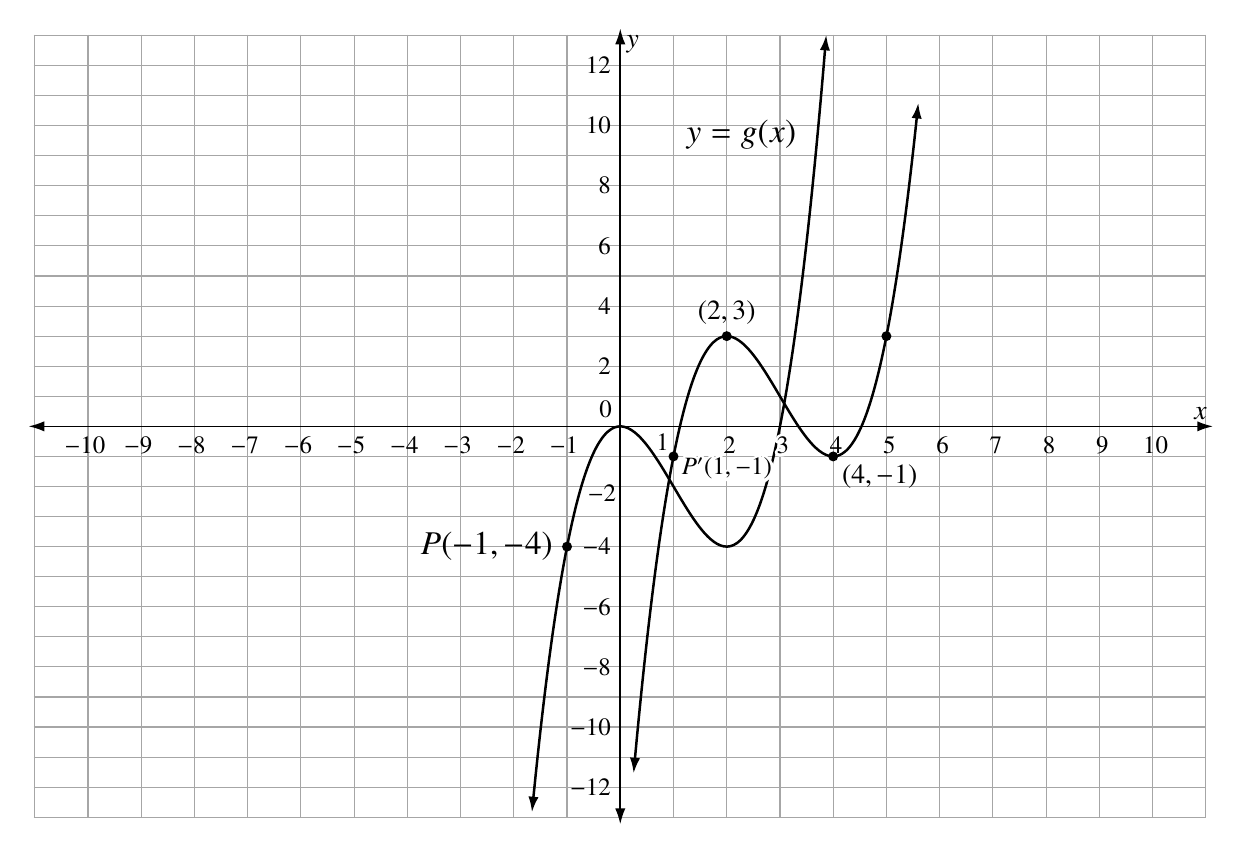
\begin{tikzpicture}[x=0.0127cm, y=-0.0127cm]
  \def\ox{604}\def\oy{420}\def\ux{53.25}\def\uy{30.08}
  \foreach \i in {-11,...,11} \draw[black!35, line width=0.4pt] ({\ox+\i*\ux},28) -- ({\ox+\i*\ux},812);
  \foreach \j in {-13,...,13} \draw[black!35, line width=0.4pt] (17,{\oy-\j*\uy}) -- (1190,{\oy-\j*\uy});
  \draw[<->] (12,\oy) -- (1197,\oy) node[above left, inner sep=2pt] {$x$};
  \draw[<->] (\ox,818) -- (\ox,22) node[below right, inner sep=2pt] {$y$};
  \foreach \i in {-10,...,-1} \node[font=\small, anchor=north, inner sep=2pt] at ({\ox+\i*\ux-3},424) {$\i$};
  \foreach \i in {2,4,5,...,10} \node[font=\small, anchor=north, inner sep=2pt] at ({\ox+\i*\ux+3},424) {$\i$};
  \node[font=\small, anchor=north east, inner sep=1pt] at ({\ox+\ux-1},424) {$1$};
  \node[font=\small, anchor=south east, inner sep=2pt] at (602,418) {$0$};
  \foreach \j in {-12,-10,-8,-6,-4,2,4,6,8,10,12} \node[font=\small, anchor=east, inner sep=2pt] at (601,{\oy-\j*\uy}) {$\j$};
  \node[font=\small, anchor=east, inner sep=0.5pt] at (602,{\oy+2*\uy+7}) {$-2$};
  % y = g(x)
  \draw[<->, line width=0.9pt, smooth, samples=90, variable=\t, domain=-1.66:3.87]
     plot ({\ox+\ux*\t},{\oy-\uy*(\t*\t*(\t-3))});
  \fill ({\ox-\ux},{\oy+4*\uy}) circle (5);
  \node[anchor=east, font=\large, inner sep=2pt] at ({\ox-\ux-8},{\oy+4*\uy}) {$P(-1,-4)$};
  \node[font=\large, anchor=east] at (790,128) {$y=g(x)$};
  % y = g(x-2)+3
  \draw[<->, line width=0.9pt, smooth, samples=90, variable=\t, domain=0.25:5.6]
     plot ({\ox+\ux*\t},{\oy-\uy*((\t-2)*(\t-2)*(\t-5)+3)});
  \foreach \p/\q in {2/3, 4/-1, 1/-1, 5/3} \fill ({\ox+\p*\ux},{\oy-\q*\uy}) circle (5);
  \node[anchor=south, inner sep=4pt] at ({\ox+2*\ux},{\oy-3*\uy}) {$(2,3)$};
  \node[anchor=north west, inner sep=1pt] at ({\ox+4.1*\ux},{\oy+1.15*\uy}) {$(4,-1)$};
  % haloed labels drawn last so the knock-out covers the curves
  \node[font=\small, anchor=north, inner sep=2pt] at ({\ox+3*\ux+3},424) {\halo{$3$}};
  \node[anchor=north west, inner sep=0pt, font=\small] at ({\ox+1.13*\ux},{\oy+1.02*\uy}) {\halo{$P'(1,-1)$}};% no room between the curves: haloed where y=g(x) crosses it
\end{tikzpicture}
\end{document}
